

\documentclass{article}
\title{Bounding parameter uncertainty in single molecule localization}
\author{C.W. Seitz}
\date{\today}

\usepackage{graphicx}
\usepackage{subfigure,epsfig,amsfonts}
\usepackage{amsmath}
\usepackage{siunitx}
\usepackage{float}
\usepackage{bm}
\usepackage{natbib}
\bibliographystyle{unsrtnat}

\begin{document}
\maketitle


\section{Bounding parameter uncertainty in single molecule localization}

\subsection{Poisson rate of a single camera pixel}

Most detectors used for imaging have many elements (pixels) so that we can record an image projected onto the detector by a system of lenses. In fluorescence imaging, this is usually a relay consisting of an objective lens and a tube lens to focus the image onto the camera. Due to diffraction, any point emitter, such as a single fluorescent molecule, will be registered as a diffraction limited spot. The profile of that spot is often described as a Gaussian point spread function

\begin{equation}
q(x,y) = \frac{1}{2\pi\sigma^{2}}\exp\left(-\frac{(x-x_{0})^{2}+(y-y_{0})^{2}}{2\sigma^{2}}\right)
\end{equation}

where $(x_0,y_0)$ defines the coordinates of a single fluorescent molecule on a detector $\mathcal{D}$. Since light is actually made up of photons, this function describes a probability density for photon arrivals in two-dimensions. Therefore, an image captured by a camera is just a histogram of photon arrivals and a discrete approximation of $q(x,y)$. If $q(x,y)$ is constant in time, and we detect a very large number of photons, the value at a pixel approaches an integral of $q(x,y)$ over the pixel:

\begin{equation}
\lambda_{k} = \gamma\cdot\int_{\mathcal{D}_{k}} q(x,y)dxdy
\end{equation}

The variable $\lambda_{k}$ at a pixel $k$ defines the probability of observing a photon per unit time and therefore we can define the number of photons arriving at each pixel as a random variable

\begin{equation*}
P(S_{k}) = \mathrm{Poisson}(\lambda_{k})
\end{equation*}


It would be convenient to obtain an analytical expression for $\lambda_{k}$ given the parameters of the point spread function $\theta = (x_0,y_0,\sigma)$. Recall first the appropriate normalization for a Gaussian function in one dimension

\begin{equation*}
\int_{-\infty}^{\infty}\exp(-\alpha x^{2}) = \sqrt{\frac{\pi}{\alpha}} \rightarrow G(x) = \sqrt{\frac{\alpha}{\pi}}\exp(-\alpha x^{2})
\end{equation*}


For the standard definition of a Gaussian with variance $\sigma^{2}$, $\alpha = \frac{1}{2\sigma^{2}}$. Suppose I pick my origin to be at $(x_{0},y_{0})$, such that pixel coordinates become $x' = x_{0} + \Delta x$ and $y' = y_{0} + \Delta y$ are the coordinates of the top left corner of a pixel

\begin{align*}
\int_{\mathcal{D}_{k}} q(x,y)dxdy &= \sqrt{\frac{\alpha}{\pi}}\int_{x'}^{x'+\Delta}dx\exp\left(-\alpha x^{2}\right) \sqrt{\frac{\alpha}{\pi}}\int_{y'}^{y' + \Delta}dy\exp\left(-\alpha y^{2}\right)\\
&=\sqrt{\frac{\alpha}{\pi}}\cdot\frac{1}{2}\left\{\mathrm{erf}((x'+\Delta)\sqrt{\alpha})-\mathrm{erf}(x'\sqrt{\alpha})\right\}\sqrt{\frac{\alpha}{\pi}}\cdot\frac{1}{2}\left\{\mathrm{erf}((y'+\Delta)\sqrt{\alpha})-\mathrm{erf}(y'\sqrt{\alpha})\right\}
\end{align*}

The (possibly cropped) detector $\mathcal{D}$ is a $M\times M$ array of square pixels of width $\Delta$ and quantum efficiency $\gamma$. Our goal is to evaluate $\lambda_{k}$ for all $\mathcal{D}_{k} \in \mathcal{D}$ according to the equation above. Therefore, we write the expression for the rate at pixel $k$ with coordinates $(x',y')$

\begin{align}
\lambda_{k} &= \frac{\gamma\alpha}{4\pi}\left\{\mathrm{erf}((x'+\Delta)\sqrt{\alpha})-\mathrm{erf}(x'\sqrt{\alpha})\right\}\left\{\mathrm{erf}((y'+\Delta)\sqrt{\alpha})-\mathrm{erf}(y'\sqrt{\alpha})\right\}
\end{align}

\subsection{Corrupting a Poisson process with white noise}

Detectors often suffer from dark noise (thermal noise) and there may also be a background signal. Considering the former first, we define another r.v. $W_{k}$ which represents Gaussian dark noise associated with pixel $k$. Unless otherwise specified we will always assume that $W_{k} \sim \mathcal{N}(m_{k},\sigma_{w,k}^{2})$. We represent our corrupted signal as another random variable $H_{k}$. As a side note, we define $S_{k}$ to have units of photons $[\mathrm{p}]$, while $H_{k}$ has units of photoelectrons $[e^{-}]$. The conversion factor between the two is the gain of the detector element $g_{k}\; [e^{-}\mathrm{p}^{-1}]$.

\vspace{0.1in}
\begin{align*}
P(S_{k},H_{k}) &= P(H_{k}|S_{k})P(S_{k})\\
&= \frac{1}{\sqrt{2\pi}\sigma}\exp\left(-\frac{(H_{k}-g_{k}n_{k}-m_{k})^{2}}{2\sigma_{k}^{2}}\right)\frac{\exp\left({-\lambda_{k}}\right)\lambda_{k}^{n_{k}}}{n_{k}!}
\end{align*}
\vspace{0.1in}

Marginalizing over $S_{k}$ gives the desired distribution over $H_{k}$

\begin{equation}
P(H_{k}) = \frac{\exp\left({-\lambda_{k}}\right)}{\sqrt{2\pi}\sigma}\sum_{n=0}^{\infty}\frac{\lambda_{k}^{n}}{n!}\exp\left(-\frac{(H_{k}-g_{k}n-m_{k})^{2}}{2\sigma_{k}^{2}}\right)
\end{equation}

\begin{figure}
\centering     %%% not \center
\subfigure[Theoretical prediction of $P(S_{k},H_{k})$ and marginal distributions for $g_{k}=1$, $\lambda_{k}=10\;\mathrm{cpms}$, and $\Delta t = 5\si{ms}$ and $\sigma_{k}=5 \;e^{-}$]{\label{fig:a}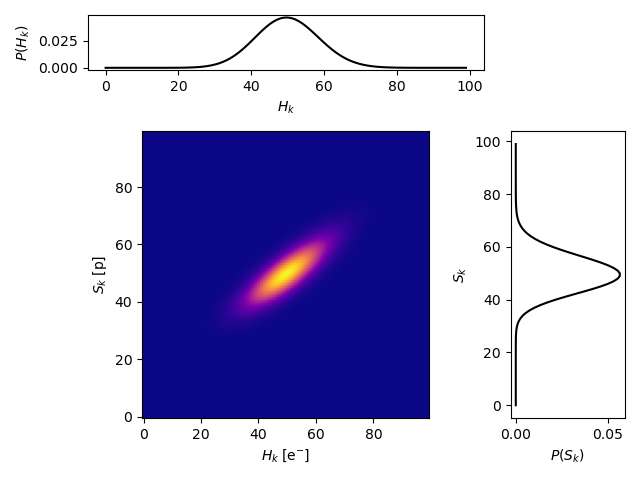
\includegraphics[width=120mm]{theoretical}}
\subfigure[Simulation of $P(S_{k},H_{k})$ and marginal distributions]{\label{fig:b}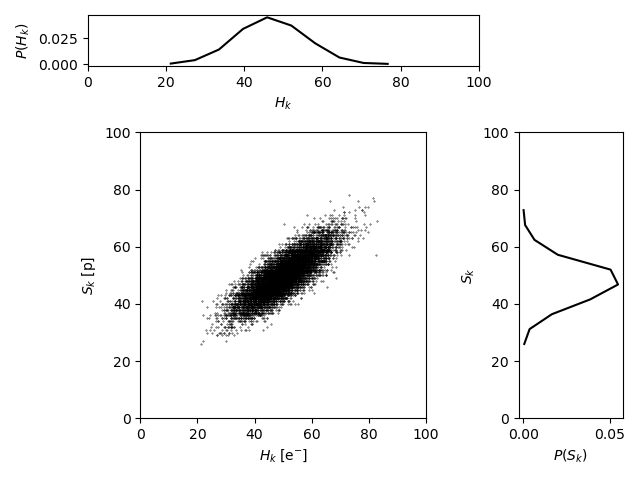
\includegraphics[width=120mm]{experimental}}

\end{figure}



\subsection{Fisher information and the Cramer-Rao bound}

Suppose we are given samples from a normal distribution with unknown parameters. We then decide to build a model normal distribution. Perhaps we define a likelihood function over the $\mu-\sigma$ plane based on a set of samples, does the likelihood of the data vary? If the likelihood surface is flat, all parameter sets would be equally likely and the data does not appear to carry much information about the parameters. If the surface has a number of bumps or inflection points, then we expect our data does carry information about the parameters. This ``bumpiness" of the likelihood surface is measured by computing the variance the second derivative of the likelihood over the parameter space\\

\vspace{0.2in}
The log-likelihood of an image under parameters $\theta = (x_{0},y_{0},\sigma^{2},\sigma_{w}^{2},g_{k})$, assuming each pixel is an independent but not identical random variable, reads

\begin{align*}
\ell(H|\theta) = \log\prod_{k}^{M^{2}} P(H_{k}|\theta) = \sum_{k=1}^{M^{2}} \ell (H_{k}|\theta)
\end{align*}


When there are many parameters, the Fisher Information (second moment of the score) is a matrix

\begin{align*}
I_{ij}(\theta) &= \underset{\theta}{\mathbb{E}}\left[\frac{\partial}{\partial\theta_{i}} \left(\ell(H|\theta)\right)\frac{\partial}{\partial\theta_{j}} \left(\ell(H|\theta)\right)\right]\\
\end{align*}

The only elements of the matrix of interest are on the diagonal, which allows us to write

\begin{align*}
I(\theta_{i}) &= \underset{\theta}{\mathbb{E}}\left[\sum_{k}\frac{\partial^{2}}{\partial\theta_{i}^{2}}  \ell (H_{k}|\theta)\right]\\
\end{align*}

At this point, we need to evaluate the second derivative w.r.t each of the parameters in $\theta = (x_{0},y_{0},\sigma^{2})$. We have shown that the model for the number of photoelectrons at a pixel is




\section{Supplement on Poisson processes}

The Poisson process can be derived very quickly by noticing that it is simply the continuous-time limit of the Binomial distribution.

\begin{align*}
B(m;t) &= {n\choose m}\lambda^{m}(1-\lambda)^{n-m}\\
\end{align*}

Since $\lambda$ is the fraction of successes, the expected number of successes is $\mu = n\lambda$

\begin{align*}
B(m;t) &=  {n\choose m}\left(\frac{\mu}{n}\right)^{m}\left(1-\frac{\mu}{n}\right)^{n-m}\\
&= {n\choose m}\left(\frac{\mu}{n}\right)^{m}\left(1-\frac{\mu}{n}\right)^{n}\left(1-\frac{\mu}{n}\right)^{-m}
\end{align*}

\begin{align*}
B(m;t) &= \frac{n!}{m!(n-m)!}\left(\frac{\mu}{n}\right)^{m}\left(1-\frac{\mu}{n}\right)^{n}\left(1-\frac{\mu}{n}\right)^{-m}\\
&= \frac{n!}{(n-m)!}\left(\frac{1}{n}\right)^{m}\left(1-\frac{\mu}{n}\right)^{-m}\frac{\mu^{m}\left(1-\frac{\mu}{n}\right)^{n}}{m!}\\
\end{align*}

In the first term, we can take the first $m$ subterms of the numerator $n! = n(n-1)...(n-m)$ and, since $n>>m$, each term will cancel with one factor of $n$ from the term $1/n^{m}$. This leaves

\begin{align*}
B(m;t) &= \frac{(n-m)!}{(n-m)!}\left(1-\frac{\mu}{n}\right)^{-m}\frac{\mu^{m}\exp(-\mu)}{m!}\\\\
\end{align*}

We now take the continuous time limit i.e. $n\rightarrow\infty$ and, again, since $m << n$ we are left with 

\begin{align*}
\underset{n\rightarrow\infty}{\mathrm{lim}} \;\; B(m;t) &= \frac{\mu^{m}\exp(-\mu)}{m!}\\
\end{align*}

If an event can be detected will probability $\gamma$, the rate of the Poisson process will be reduced by that factor i.e., $\lambda' = \gamma\lambda$. Therefore, the mean and variance of the process becomes $\mu = \gamma\lambda\Delta t$



\end{document}